\documentclass[aspectratio=169]{beamer}
\usetheme{Madrid}
\usecolortheme{default}

\usepackage[utf8]{inputenc}
\usepackage{listings}
\usepackage{xcolor}
\usepackage{tikz}
\usepackage{graphicx}
\usetikzlibrary{positioning,shapes,arrows,calc,matrix,backgrounds}

% Python code configuration
\lstset{
    language=Python,
    basicstyle=\ttfamily\tiny,
    keywordstyle=\color{blue},
    commentstyle=\color{green!60!black},
    stringstyle=\color{red},
    showstringspaces=false,
    breaklines=true,
    frame=single,
    numbers=left,
    numberstyle=\tiny\color{gray}
}

\title{Python for Machine Learning}
\subtitle{The Essential Tools}
\author{Meyssem Bouzaien}
\institute{Academic Year: 2025 - 2026}
\date{}

\begin{document}

\frame{\titlepage}

\begin{frame}{Course Outline}
\tableofcontents
\end{frame}

%% ========== SECTION 1 ==========
\section{Introduction and Environment}

\begin{frame}{Course Objectives}
\begin{block}{What you will learn}
\begin{itemize}
    \item Master NumPy, Pandas, Matplotlib, and Scikit-learn
    \item Manipulate and prepare real-world data
    \item Visualize your results
    \item Build your first ML model
\end{itemize}
\end{block}


\end{frame}

\begin{frame}{Working Environment: You Have a Choice!}
\begin{columns}[T]
\column{0.48\textwidth}
\textbf{Available options:}
\begin{itemize}
    \item \alert{Google Colab} (recommended)
    \item Jupyter Notebook
    \item Anaconda + Jupyter
    \item VS Code
    \item PyCharm
\end{itemize}

\column{0.48\textwidth}
\begin{block}{Why Google Colab?}
\begin{itemize}
    \item Free
    \item No installation
    \item GPU available
    \item Easy to share
\end{itemize}
\end{block}
\end{columns}

\vspace{0.4cm}
\footnotesize{\textit{Use whichever environment you prefer!}}
\end{frame}

\begin{frame}{The 4 Essential Libraries}
\begin{center}
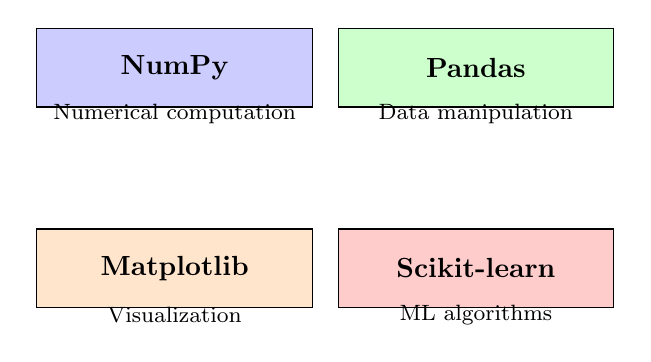
\begin{tikzpicture}[scale=0.85]
    \node[draw, rectangle, fill=blue!20, minimum width=3.5cm, minimum height=1cm] at (0,3) {\textbf{NumPy}};
    \node[text width=3.5cm, align=center, font=\footnotesize] at (0,2.3) {Numerical computation};
    
    \node[draw, rectangle, fill=green!20, minimum width=3.5cm, minimum height=1cm] at (4.5,3) {\textbf{Pandas}};
    \node[text width=3.5cm, align=center, font=\footnotesize] at (4.5,2.3) {Data manipulation};
    
    \node[draw, rectangle, fill=orange!20, minimum width=3.5cm, minimum height=1cm] at (0,0) {\textbf{Matplotlib}};
    \node[text width=3.5cm, align=center, font=\footnotesize] at (0,-0.7) {Visualization};
    
    \node[draw, rectangle, fill=red!20, minimum width=3.5cm, minimum height=1cm] at (4.5,0) {\textbf{Scikit-learn}};
    \node[text width=3.5cm, align=center, font=\footnotesize] at (4.5,-0.7) {ML algorithms};
\end{tikzpicture}
\end{center}
\end{frame}

%% ========== SECTION 2 ==========
\section{NumPy - Numerical Computation}

\begin{frame}{NumPy: What Exactly Is It?}
\begin{block}{Definition}
NumPy (Numerical Python) is the fundamental library for scientific computing in Python. It provides high-performance data structures for working with multidimensional arrays.
\end{block}

\vspace{0.3cm}
\begin{columns}[T]
\column{0.48\textwidth}
\textbf{Characteristics:}
\begin{itemize}
    \item N-dimensional arrays
    \item Vectorized operations
    \item Optimized in C
    \item Foundation for Pandas, Scikit-learn
\end{itemize}

\column{0.48\textwidth}
\textbf{Data types:}
\begin{itemize}
    \item int32, int64
    \item float32, float64
    \item bool, complex
    \item Homogeneous within an array
\end{itemize}
\end{columns}
\end{frame}

\begin{frame}[fragile]{NumPy: Why?}
\begin{columns}[T]
\column{0.48\textwidth}
\textbf{Python lists:}
\begin{lstlisting}
my_list = [1, 2, 3, 4]
result = []
for x in my_list:
    result.append(x * 2)
# Slow!
\end{lstlisting}

\column{0.48\textwidth}
\textbf{NumPy arrays:}
\begin{lstlisting}
import numpy as np
array = np.array([1,2,3,4])
result = array * 2
# Fast!
\end{lstlisting}
\end{columns}

\vspace{0.5cm}
\begin{block}{NumPy Advantages}
\begin{itemize}
    \item 50-100x faster than lists
    \item Simple syntax
    \item Less memory usage
\end{itemize}
\end{block}
\end{frame}

\begin{frame}{1D vs 2D vs 3D Arrays - Visualization}
\begin{center}
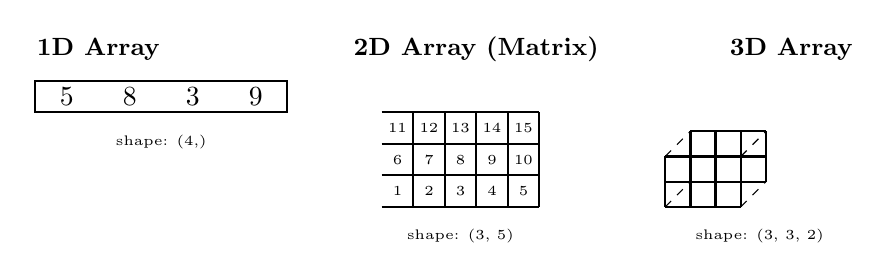
\begin{tikzpicture}[scale=0.8]
    % 1D Array
    \node[font=\small\bfseries] at (-2,3) {1D Array};
    \draw[thick] (-3,2) rectangle (1,2.5);
    \foreach \i/\val in {0/5, 1/8, 2/3, 3/9}
        \node at (-2.5+\i,2.25) {\val};
    \node[below, font=\tiny] at (-1,1.8) {shape: (4,)};
    
    % 2D Array
    \node[font=\small\bfseries] at (4,3) {2D Array (Matrix)};
    \draw[thick, fill=blue!10] (2.5,0.5) grid[step=0.5] (5,2);
    \foreach \i/\j/\val in {0/0/1, 1/0/2, 2/0/3, 3/0/4, 4/0/5,
                            0/1/6, 1/1/7, 2/1/8, 3/1/9, 4/1/10,
                            0/2/11, 1/2/12, 2/2/13, 3/2/14, 4/2/15}
        \node[font=\tiny] at (2.75+\i*0.5,0.75+\j*0.5) {\val};
    \node[below, font=\tiny] at (3.75,0.3) {shape: (3, 5)};
    
    % 3D Array
    \node[font=\small\bfseries] at (9,3) {3D Array};
    \begin{scope}[shift={(7,0.5)}]
        \draw[thick, fill=red!20] (0,0) grid[step=0.4] (1.2,0.8);
        \draw[thick, fill=red!30] (0.2,0.2) grid[step=0.4] (1.4,1);
        \draw[thick, fill=red!40] (0.4,0.4) grid[step=0.4] (1.6,1.2);
        \draw[dashed] (0,0) -- (0.4,0.4);
        \draw[dashed] (1.2,0) -- (1.6,0.4);
        \draw[dashed] (0,0.8) -- (0.4,1.2);
        \draw[dashed] (1.2,0.8) -- (1.6,1.2);
    \end{scope}
    \node[below, font=\tiny] at (8.5,0.3) {shape: (3, 3, 2)};
\end{tikzpicture}
\end{center}
\end{frame}

\begin{frame}[fragile]{Creating Arrays}
\begin{lstlisting}
import numpy as np

# From a list
a = np.array([1, 2, 3, 4, 5])
print(a)  # [1 2 3 4 5]

# 2D matrix
m = np.array([[1, 2, 3],
              [4, 5, 6]])
print(m.shape)  # (2, 3)

# Special arrays
zeros = np.zeros((3, 4))        # Matrix of zeros
ones = np.ones((2, 3))          # Matrix of ones
range_arr = np.arange(0, 10, 2) # [0 2 4 6 8]
linear = np.linspace(0, 1, 5)   # 5 values [0, 0.25, 0.5, 0.75, 1]
random = np.random.rand(3, 3)   # Random values in [0, 1)
\end{lstlisting}
\end{frame}

\begin{frame}[fragile]{Dimensions and Shapes}
\begin{columns}[T]
\column{0.55\textwidth}
\begin{lstlisting}
data = np.array([[1, 2, 3, 4],
                 [5, 6, 7, 8],
                 [9, 10, 11, 12]])

print(data.shape)  # (3, 4)
print(data.ndim)   # 2
print(data.size)   # 12
print(data.dtype)  # int64
\end{lstlisting}

\column{0.42\textwidth}
\begin{center}
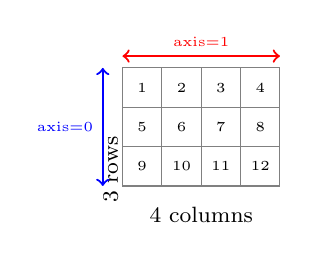
\begin{tikzpicture}[scale=0.5]
    \draw[step=1cm,gray,thin] (0,0) grid (4,3);
    \foreach \i in {0,...,2}
        \foreach \j in {0,...,3}
            \node[font=\tiny] at (\j+0.5,2.5-\i) {\the\numexpr\i*4+\j+1\relax};
    \node[below, font=\footnotesize] at (2,-0.3) {4 columns};
    \node[left, rotate=90, font=\footnotesize] at (-0.3,1.5) {3 rows};
    
    \draw[<->, thick, red] (0,3.3) -- (4,3.3);
    \node[above, red, font=\tiny] at (2,3.3) {axis=1};
    \draw[<->, thick, blue] (-0.5,0) -- (-0.5,3);
    \node[left, blue, font=\tiny] at (-0.5,1.5) {axis=0};
\end{tikzpicture}
\end{center}
\end{columns}

\vspace{0.3cm}
\begin{alertblock}{Important}
\textbf{axis=0}: operations across rows (vertical) \\
\textbf{axis=1}: operations across columns (horizontal)
\end{alertblock}
\end{frame}

\begin{frame}{Broadcasting - Visual Concept}
\begin{center}
\textbf{How NumPy operates on arrays of different sizes}

\vspace{0.3cm}
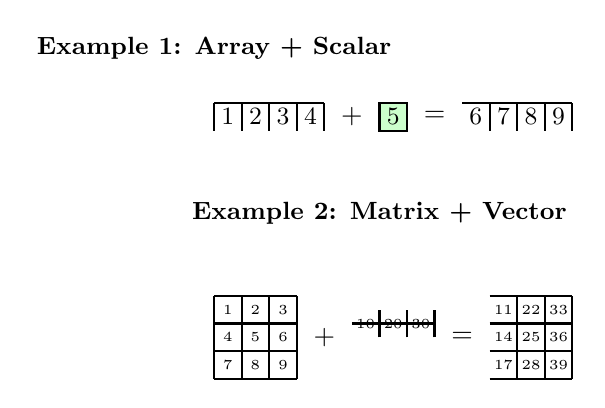
\begin{tikzpicture}[scale=0.7]
    \node[font=\small\bfseries] at (0,3.5) {Example 1: Array + Scalar};
    
    \draw[thick, fill=blue!20] (0,2) grid[step=0.5] (2,2.5);
    \foreach \i/\val in {0/1, 1/2, 2/3, 3/4}
        \node[font=\small] at (0.25+\i*0.5,2.25) {\val};
    
    \node at (2.5,2.25) {$+$};
    
    \draw[thick, fill=green!20] (3,2) rectangle (3.5,2.5);
    \node[font=\small] at (3.25,2.25) {5};
    
    \node at (4,2.25) {$=$};
    
    \draw[thick, fill=orange!20] (4.5,2) grid[step=0.5] (6.5,2.5);
    \foreach \i/\val in {0/6, 1/7, 2/8, 3/9}
        \node[font=\small] at (4.75+\i*0.5,2.25) {\val};
    
    \node[font=\small\bfseries] at (3,0.5) {Example 2: Matrix + Vector};
    
    \draw[thick, fill=blue!20] (0,-1) grid[step=0.5] (1.5,-2.5);
    \foreach \i/\j/\val in {0/0/1, 1/0/2, 2/0/3,
                            0/1/4, 1/1/5, 2/1/6,
                            0/2/7, 1/2/8, 2/2/9}
        \node[font=\tiny] at (0.25+\i*0.5,-1.25-\j*0.5) {\val};
    
    \node at (2,-1.75) {$+$};
    
    \draw[thick, fill=green!20] (2.5,-1.25) grid[step=0.5] (4,-1.75);
    \foreach \i/\val in {0/10, 1/20, 2/30}
        \node[font=\tiny] at (2.75+\i*0.5,-1.5) {\val};
    
    \node at (4.5,-1.75) {$=$};
    
    \draw[thick, fill=orange!20] (5,-1) grid[step=0.5] (6.5,-2.5);
    \foreach \i/\j/\val in {0/0/11, 1/0/22, 2/0/33,
                            0/1/14, 1/1/25, 2/1/36,
                            0/2/17, 1/2/28, 2/2/39}
        \node[font=\tiny] at (5.25+\i*0.5,-1.25-\j*0.5) {\val};
\end{tikzpicture}
\end{center}
\end{frame}

\begin{frame}[fragile]{Mathematical Operations}
\begin{columns}[T]
\column{0.48\textwidth}
\textbf{Basic operations:}
\begin{lstlisting}
a = np.array([1,2,3,4])
b = np.array([10,20,30,40])

a + b  # [11 22 33 44]
a * b  # [10 40 90 160]
a ** 2 # [1 4 9 16]
a / 2  # [0.5 1 1.5 2]
\end{lstlisting}

\column{0.48\textwidth}
\textbf{Useful functions:}
\begin{lstlisting}
data = np.array([1,2,3,4,5])

np.mean(data)  # 3.0
np.sum(data)   # 15
np.min(data)   # 1
np.max(data)   # 5
np.std(data)   # Standard deviation
np.sqrt(data)  # Square roots
np.median(data) # Median
\end{lstlisting}
\end{columns}

\vspace{0.3cm}
\begin{alertblock}{Important}
All operations are performed element-wise!
\end{alertblock}
\end{frame}

\begin{frame}{Indexing - Visualization}
\begin{center}
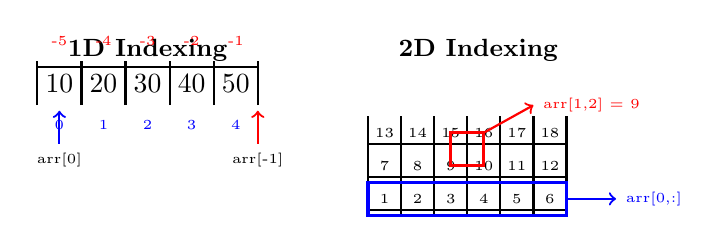
\begin{tikzpicture}[scale=0.7]
    \node[font=\small\bfseries] at (2,3.5) {1D Indexing};
    \draw[thick] (0,2.5) grid[step=0.8] (4,3.3);
    \foreach \i/\val in {0/10, 1/20, 2/30, 3/40, 4/50}
        \node at (0.4+\i*0.8,2.9) {\val};
    
    \foreach \i in {0,...,4}
        \node[below, font=\tiny, blue] at (0.4+\i*0.8,2.4) {\i};
    
    \foreach \i/\val in {0/-5, 1/-4, 2/-3, 3/-2, 4/-1}
        \node[above, font=\tiny, red] at (0.4+\i*0.8,3.4) {\val};
    
    \draw[->, thick, blue] (0.4,1.8) -- (0.4,2.4);
    \node[below, font=\tiny] at (0.4,1.8) {arr[0]};
    
    \draw[->, thick, red] (4,1.8) -- (4,2.4);
    \node[below, font=\tiny] at (4,1.8) {arr[-1]};
    
    \node[font=\small\bfseries] at (8,3.5) {2D Indexing};
    \draw[thick, fill=blue!10] (6,0.5) grid[step=0.6] (9.6,2.3);
    \foreach \i/\j/\val in {0/0/1, 1/0/2, 2/0/3, 3/0/4, 4/0/5, 5/0/6,
                            0/1/7, 1/1/8, 2/1/9, 3/1/10, 4/1/11, 5/1/12,
                            0/2/13, 1/2/14, 2/2/15, 3/2/16, 4/2/17, 5/2/18}
        \node[font=\tiny] at (6.3+\i*0.6,0.8+\j*0.6) {\val};
    
    \draw[red, very thick] (7.5,1.4) rectangle (8.1,2);
    \draw[->, red, thick] (8.1,2) -- (9,2.5);
    \node[right, red, font=\tiny] at (9,2.5) {arr[1,2] = 9};
    
    \draw[blue, very thick] (6,0.5) rectangle (9.6,1.1);
    \draw[->, blue, thick] (9.6,0.8) -- (10.5,0.8);
    \node[right, blue, font=\tiny] at (10.5,0.8) {arr[0,:]};
\end{tikzpicture}
\end{center}
\end{frame}

\begin{frame}[fragile]{Indexing and Slicing}
\begin{lstlisting}
# 1D Array
arr = np.array([10, 20, 30, 40, 50])
arr[0]    # 10 - first element
arr[-1]   # 50 - last element
arr[1:4]  # [20 30 40] - slicing

# 2D Array
mat = np.array([[1, 2, 3],
                [4, 5, 6],
                [7, 8, 9]])

mat[0, 0]     # 1 - first row, first column
mat[1, :]     # [4 5 6] - the whole row 1
mat[:, 2]     # [3 6 9] - the whole column 2
mat[0:2, 1:3] # [[2 3]    - sub-matrix
              #  [5 6]]
\end{lstlisting}
\end{frame}

\begin{frame}[fragile]{NumPy Practice Exercise}
\begin{block}{Your turn!}
\begin{enumerate}
    \item Create an array of 20 random numbers between 0 and 100
    \item Compute the mean and standard deviation
    \item Find the values greater than 50
    \item Create a 5x4 matrix of random numbers
    \item Compute the sum of each column
\end{enumerate}
\end{block}

\begin{lstlisting}
# Hint to get started
import numpy as np

# Generate random numbers
data = np.random.randint(0, 100, 20)
\end{lstlisting}
\end{frame}

%% ========== SECTION 3 ==========
\section{Pandas - Data Manipulation}

\begin{frame}{Pandas: What Is It?}
\begin{block}{DataFrame = an Excel spreadsheet in Python}
\begin{itemize}
    \item Tabular data structure
    \item Named columns
    \item Indexed rows
    \item Mixed data types
\end{itemize}
\end{block}

\vspace{0.3cm}
\begin{center}
\begin{tabular}{|c|c|c|c|}
\hline
\textbf{Name} & \textbf{Age} & \textbf{City} & \textbf{Score} \\
\hline
Alice & 25 & Paris & 85 \\
Bob & 30 & Lyon & 92 \\
Charlie & 22 & Marseille & 78 \\
\hline
\end{tabular}
\end{center}

\vspace{0.3cm}
\textit{This is how we work with data in ML!}
\end{frame}

\begin{frame}[fragile]{Creating a DataFrame (1/2)}
\begin{lstlisting}
import pandas as pd

# Method 1: From a dictionary
data = {
    'Name': ['Alice', 'Bob', 'Charlie'],
    'Age': [25, 30, 22],
    'City': ['Paris', 'Lyon', 'Marseille'],
    'Score': [85, 92, 78]
}
df = pd.DataFrame(data)
print(df)
\end{lstlisting}

\vspace{0.2cm}
\begin{lstlisting}[numbers=none,frame=none]
       Name  Age       City  Score
0    Alice   25      Paris     85
1      Bob   30       Lyon     92
2  Charlie   22  Marseille     78
\end{lstlisting}
\end{frame}

\begin{frame}[fragile]{Creating a DataFrame (2/2)}
\textbf{Loading from a CSV file:}
\begin{lstlisting}
import pandas as pd

# From a CSV file
df = pd.read_csv('data.csv')

# From an Excel file
df = pd.read_excel('data.xlsx')

# From a URL
url = 'https://example.com/data.csv'
df = pd.read_csv(url)
\end{lstlisting}

\vspace{0.3cm}
\textbf{First things to check:}
\begin{lstlisting}
df.head()      # first 5 rows
df.tail()      # last 5 rows
df.shape       # (rows, columns)
df.info()      # column info
df.describe()  # statistics
\end{lstlisting}
\end{frame}

\begin{frame}[fragile]{Exploring the Data}
\begin{lstlisting}
# Load the Iris dataset
df = pd.read_csv('iris.csv')

# Dimensions
print(df.shape)  # (150, 5)

# Column names
print(df.columns)

# Data types
print(df.dtypes)

# Descriptive statistics
print(df.describe())

# Count unique values
print(df['species'].value_counts())

# Check for missing values
print(df.isnull().sum())
\end{lstlisting}
\end{frame}

\begin{frame}[fragile]{Selecting Data (1/2)}
\begin{lstlisting}
# Select a column
ages = df['Age']
# or
ages = df.Age

# Select several columns
subset = df[['Name', 'Score']]

# Filter rows
successful_students = df[df['Score'] > 80]

# Multiple conditions
filtered = df[(df['Age'] > 20) & (df['Score'] > 85)]
\end{lstlisting}
\end{frame}

\begin{frame}[fragile]{Selecting Data (2/2)}
\begin{lstlisting}
# Select by position (iloc)
df.iloc[0]        # first row
df.iloc[0:3]      # first 3 rows
df.iloc[0:3, 0:2] # 3 rows, 2 columns

# Select by label (loc)
df.loc[0, 'Name']            # specific value
df.loc[0:2, ['Name', 'Age']] # mixed selection
\end{lstlisting}

\vspace{0.3cm}
\begin{block}{iloc vs loc}
\begin{itemize}
    \item \textbf{iloc}: uses positions (0, 1, 2...)
    \item \textbf{loc}: uses labels/names
\end{itemize}
\end{block}
\end{frame}

\begin{frame}[fragile]{Operations on Data}
\begin{lstlisting}
# Add a new column
df['Double_Score'] = df['Score'] * 2

# Modify a column
df['Age'] = df['Age'] + 1

# Drop a column
df = df.drop('Double_Score', axis=1)

# Drop a row
df = df.drop(0, axis=0)

# Sort the data
df_sorted = df.sort_values('Score', ascending=False)

# Group and aggregate
averages = df.groupby('City')['Score'].mean()
\end{lstlisting}
\end{frame}

\begin{frame}[fragile]{Handling Missing Values}
\begin{lstlisting}
# Check missing values
print(df.isnull().sum())

# Drop rows with missing values
df_clean = df.dropna()

# Drop columns with missing values
df_clean = df.dropna(axis=1)

# Fill with a value
df_filled = df.fillna(0)

# Fill with the mean
df['Age'] = df['Age'].fillna(df['Age'].mean())

# Fill with the previous value
df_filled = df.fillna(method='ffill')
\end{lstlisting}
\end{frame}

\begin{frame}[fragile]{Pandas Practice Exercise}
\begin{block}{Iris Dataset}
\begin{enumerate}
    \item Load iris.csv
    \item Display the first 10 rows
    \item How many rows and columns are there?
    \item Which species are present?
    \item Compute the mean of each numeric column
    \item Filter flowers with sepal\_length > 6
    \item Create: sepal\_area = sepal\_length * sepal\_width
\end{enumerate}
\end{block}

\begin{lstlisting}
import pandas as pd
# Your code here...
\end{lstlisting}
\end{frame}

%% ========== NEW SECTION: CORRELATION ==========
\section{Understanding Correlation}

\begin{frame}{What is Correlation? (1/3)}
\begin{block}{Definition}
Correlation measures the \textbf{linear relationship} between two quantitative variables.\\
It ranges between \textbf{-1} and \textbf{+1}.
\end{block}

\vspace{0.3cm}

\begin{center}
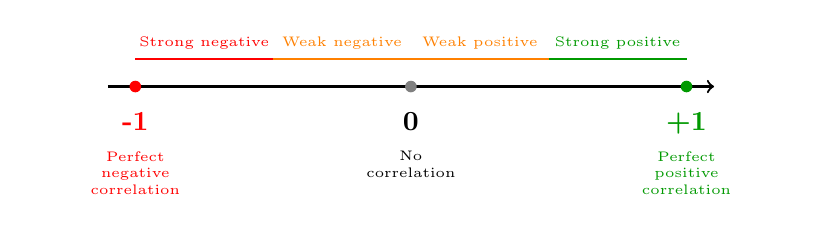
\begin{tikzpicture}[scale=0.7]
    \draw[->, thick] (-5.5,0) -- (5.5,0);
    
    \fill[red] (-5,0) circle (3pt);
    \node[below, red] at (-5,-0.3) {\textbf{-1}};
    \node[below, red, text width=2.5cm, align=center, font=\tiny] at (-5,-1) {Perfect\\negative\\correlation};
    
    \fill[gray] (0,0) circle (3pt);
    \node[below] at (0,-0.3) {\textbf{0}};
    \node[below, text width=2cm, align=center, font=\tiny] at (0,-1) {No\\correlation};
    
    \fill[green!60!black] (5,0) circle (3pt);
    \node[below, green!60!black] at (5,-0.3) {\textbf{+1}};
    \node[below, green!60!black, text width=2.5cm, align=center, font=\tiny] at (5,-1) {Perfect\\positive\\correlation};
    
    \draw[red, thick] (-5,0.5) -- (-2.5,0.5);
    \node[above, red, font=\tiny] at (-3.75,0.5) {Strong negative};
    
    \draw[orange, thick] (-2.5,0.5) -- (0,0.5);
    \node[above, orange, font=\tiny] at (-1.25,0.5) {Weak negative};
    
    \draw[orange, thick] (0,0.5) -- (2.5,0.5);
    \node[above, orange, font=\tiny] at (1.25,0.5) {Weak positive};
    
    \draw[green!60!black, thick] (2.5,0.5) -- (5,0.5);
    \node[above, green!60!black, font=\tiny] at (3.75,0.5) {Strong positive};
\end{tikzpicture}
\end{center}
\end{frame}

\begin{frame}{What is Correlation? (2/3)}
\textbf{Interpreting the values:}

\vspace{0.2cm}

\begin{center}
\small
\begin{tabular}{|c|l|l|}
\hline
\textbf{Value} & \textbf{Strength} & \textbf{Meaning} \\
\hline
\textcolor{green!60!black}{+0.90 to +1.00} & Very strong + & Both increase together \\
\textcolor{green!60!black}{+0.70 to +0.89} & Strong + & Clear relationship \\
\textcolor{orange}{+0.40 to +0.69} & Moderate + & Visible trend \\
\textcolor{orange}{+0.10 to +0.39} & Weak + & Slight relationship \\
\textcolor{gray}{-0.09 to +0.09} & Negligible & No relationship \\
\textcolor{orange}{-0.10 to -0.39} & Weak - & Slight inverse relationship \\
\textcolor{red}{-0.40 to -0.69} & Moderate - & Inverse trend \\
\textcolor{red}{-0.70 to -0.89} & Strong - & Clear inverse relationship \\
\textcolor{red}{-0.90 to -1.00} & Very strong - & One rises, the other falls \\
\hline
\end{tabular}
\end{center}
\end{frame}

\begin{frame}{What is Correlation? (3/3)}
\textbf{Visual examples:}

\begin{center}
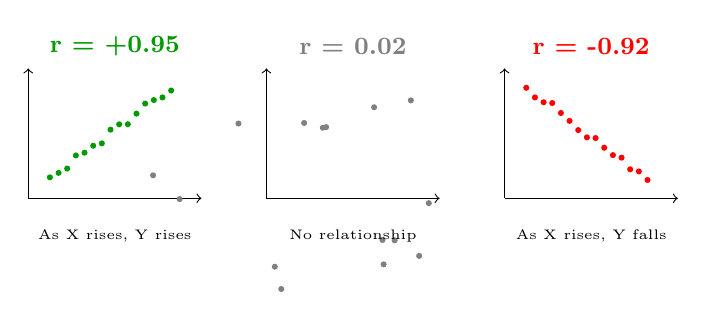
\begin{tikzpicture}[scale=0.55]
    % Strong positive
    \node[font=\small\bfseries, green!60!black] at (2,3.5) {r = +0.95};
    \draw[->] (0,0) -- (4,0);
    \draw[->] (0,0) -- (0,3);
    \foreach \i in {1,...,15} {
        \pgfmathsetmacro{\x}{0.3+\i*0.2}
        \pgfmathsetmacro{\y}{0.3+\i*0.15+rand*0.1}
        \fill[green!60!black] (\x,\y) circle (2pt);
    }
    \node[below, font=\tiny] at (2,-0.5) {As X rises, Y rises};
    
    % No correlation
    \begin{scope}[shift={(5.5,0)}]
    \node[font=\small\bfseries, gray] at (2,3.5) {r = 0.02};
    \draw[->] (0,0) -- (4,0);
    \draw[->] (0,0) -- (0,3);
    \foreach \i in {1,...,15} {
        \pgfmathsetmacro{\x}{0.3+rand*3.5}
        \pgfmathsetmacro{\y}{0.3+rand*2.5}
        \fill[gray] (\x,\y) circle (2pt);
    }
    \node[below, font=\tiny] at (2,-0.5) {No relationship};
    \end{scope}
    
    % Strong negative
    \begin{scope}[shift={(11,0)}]
    \node[font=\small\bfseries, red] at (2,3.5) {r = -0.92};
    \draw[->] (0,0) -- (4,0);
    \draw[->] (0,0) -- (0,3);
    \foreach \i in {1,...,15} {
        \pgfmathsetmacro{\x}{0.3+\i*0.2}
        \pgfmathsetmacro{\y}{2.7-\i*0.15+rand*0.1}
        \fill[red] (\x,\y) circle (2pt);
    }
    \node[below, font=\tiny] at (2,-0.5) {As X rises, Y falls};
    \end{scope}
\end{tikzpicture}
\end{center}

\vspace{0.3cm}
\begin{alertblock}{Important}
Correlation does NOT mean causation!\\
Two variables can be correlated without one causing the other.
\end{alertblock}
\end{frame}

%% ========== SECTION 4 ==========
\section{Matplotlib - Visualization}

\begin{frame}{Why Visualize?}
\begin{columns}[T]
\column{0.5\textwidth}
\textbf{A picture is worth 1000 words}
\begin{itemize}
    \item Understand the data
    \item Detect patterns
    \item Identify outliers
    \item Communicate results
    \item Verify hypotheses
\end{itemize}

\column{0.48\textwidth}
\begin{center}
\begin{tikzpicture}[scale=0.7]
    \draw[->] (0,0) -- (4,0) node[right, font=\tiny] {x};
    \draw[->] (0,0) -- (0,3) node[above, font=\tiny] {y};
    \draw[blue, thick, domain=0:3.5, samples=50] plot (\x, {0.5*\x*\x - 0.2*\x + 0.5});
    \node[font=\footnotesize] at (2,-0.7) {Visible trend!};
\end{tikzpicture}
\end{center}
\end{columns}

\vspace{0.5cm}
\begin{alertblock}{In ML}
Visualization is essential!
\end{alertblock}
\end{frame}

\begin{frame}[fragile]{Your First Plot}
\begin{lstlisting}
import matplotlib.pyplot as plt

# Data
x = [1, 2, 3, 4, 5]
y = [2, 4, 6, 8, 10]

# Create the plot
plt.plot(x, y)

# Customize
plt.xlabel('X axis')
plt.ylabel('Y axis')
plt.title('My first plot')

# Show
plt.show()
\end{lstlisting}

\vspace{0.2cm}
\textit{Simple and effective!}
\end{frame}

\begin{frame}{Iris Dataset - Overview}
\begin{columns}[T]
\column{0.5\textwidth}
\textbf{4 Features:}
\begin{itemize}
    \item sepal\_length: Sepal length
    \item sepal\_width: Sepal width
    \item petal\_length: Petal length
    \item petal\_width: Petal width
\end{itemize}

\vspace{0.3cm}
\textbf{3 Species:}
\begin{itemize}
    \item Setosa
    \item Versicolor
    \item Virginica
\end{itemize}

\column{0.48\textwidth}
\begin{center}
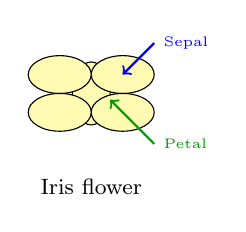
\begin{tikzpicture}[scale=0.8]
    \draw[fill=yellow!30] (0,0) ellipse (0.3 and 0.5);
    \draw[fill=yellow!30] (0.5,0.3) ellipse (0.5 and 0.3);
    \draw[fill=yellow!30] (0.5,-0.3) ellipse (0.5 and 0.3);
    \draw[fill=yellow!30] (-0.5,0.3) ellipse (0.5 and 0.3);
    \draw[fill=yellow!30] (-0.5,-0.3) ellipse (0.5 and 0.3);
    
    \draw[->, thick, blue] (1,0.8) -- (0.5,0.3);
    \node[right, blue, font=\tiny] at (1,0.8) {Sepal};
    
    \draw[->, thick, green!60!black] (1,-0.8) -- (0.3,-0.1);
    \node[right, green!60!black, font=\tiny] at (1,-0.8) {Petal};
    
    \node[below, font=\footnotesize] at (0,-1.2) {Iris flower};
\end{tikzpicture}
\end{center}
\end{columns}

\vspace{0.3cm}
\begin{block}{Goal}
Predict the species from the 4 measurements
\end{block}
\end{frame}

\begin{frame}{Iris - Correlation Matrix}
\vspace{-0.2cm}

\begin{center}
\includegraphics[width=0.55\textwidth]{iris_correlation.png}
\end{center}

\begin{block}{Key Observations}
\begin{itemize}
    \item \textbf{+0.96}: petal\_length with petal\_width (very strong!)
    \item \textbf{+0.87}: sepal\_length with petal\_length (strong)
    \item \textbf{-0.43}: sepal\_width with petal\_length (moderate negative)
\end{itemize}
\end{block}
\end{frame}

\begin{frame}{Iris - Visual Relationships}
\begin{center}
\includegraphics[width=0.95\textwidth]{iris_scatterplots.png}
\end{center}

\begin{block}{What Do We See?}
\textbf{Left:} weak correlation (-0.12) - scattered points\\
\textbf{Right:} very strong correlation (+0.96) - clear alignment!
\end{block}
\end{frame}

\begin{frame}{Iris - Histograms by Feature}
\vspace{-0.2cm}
\begin{center}
\includegraphics[width=0.6\textwidth]{iris_histograms.png}
\end{center}

\begin{block}{Observations}
Each feature has a different distribution — important for ML!
\end{block}
\end{frame}

\begin{frame}{Iris - Boxplots by Species}
\vspace{-0.2cm}

\begin{center}
\includegraphics[width=0.6\textwidth]{iris_boxplots.png}
\end{center}
\vspace{-0.2cm}

\begin{block}{Observations}
The species are well separated on petal\_length and petal\_width!
\end{block}
\end{frame}

\begin{frame}[fragile]{Chart Types - Scatter Plot}
\begin{columns}[T]
\column{0.48\textwidth}
\textbf{Code:}
\begin{lstlisting}
import matplotlib.pyplot as plt

x = [1, 2, 3, 8]
y = [1, 4, 5, 3]

plt.scatter(x, y)
plt.xlabel('X')
plt.ylabel('Y')
plt.title('Scatter plot')
plt.show()
\end{lstlisting}

\column{0.48\textwidth}
\textbf{Result:}
\begin{center}
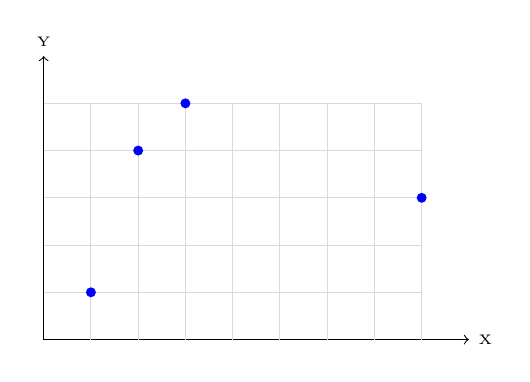
\begin{tikzpicture}[scale=0.6]
    \draw[->] (0,0) -- (9,0) node[right, font=\tiny] {X};
    \draw[->] (0,0) -- (0,6) node[above, font=\tiny] {Y};
    
    \foreach \x in {1,...,8}
        \draw[gray!30] (\x,0) -- (\x,5);
    \foreach \y in {1,...,5}
        \draw[gray!30] (0,\y) -- (8,\y);
    
    \fill[blue] (1,1) circle (3pt);
    \fill[blue] (2,4) circle (3pt);
    \fill[blue] (3,5) circle (3pt);
    \fill[blue] (8,3) circle (3pt);
\end{tikzpicture}
\end{center}
\end{columns}
\end{frame}

\begin{frame}[fragile]{Chart Types - Line Plot}
\begin{columns}[T]
\column{0.48\textwidth}
\textbf{Code:}
\begin{lstlisting}
import matplotlib.pyplot as plt

x = [1, 2, 3, 8]
y = [0, 4, 5, 3]

plt.plot(x, y)
plt.xlabel('X')
plt.ylabel('Y')
plt.title('Line plot')
plt.show()
\end{lstlisting}

\column{0.48\textwidth}
\textbf{Result:}
\begin{center}
\begin{tikzpicture}[scale=0.6]
    \draw[->] (0,0) -- (9,0) node[right, font=\tiny] {X};
    \draw[->] (0,0) -- (0,6) node[above, font=\tiny] {Y};
    
    \draw[blue, thick] (1,0) -- (2,4) -- (3,5) -- (8,3);
\end{tikzpicture}
\end{center}
\end{columns}
\end{frame}

\begin{frame}[fragile]{Chart Types - Histogram}
\begin{columns}[T]
\column{0.48\textwidth}
\textbf{Code:}
\begin{lstlisting}
import matplotlib.pyplot as plt
import numpy as np

data = np.random.randn(1000)

plt.hist(data, bins=20, 
         color='blue', 
         alpha=0.7)
plt.xlabel('Value')
plt.ylabel('Frequency')
plt.title('Histogram')
plt.show()
\end{lstlisting}

\column{0.48\textwidth}
\textbf{Result:}
\begin{center}
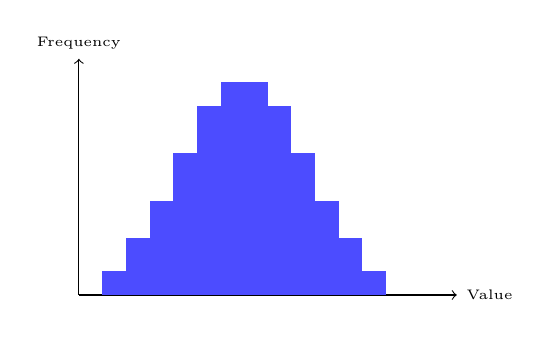
\begin{tikzpicture}[scale=0.6]
    \draw[->] (0,0) -- (8,0) node[right, font=\tiny] {Value};
    \draw[->] (0,0) -- (0,5) node[above, font=\tiny] {Frequency};
    
    \fill[blue!70] (0.5,0) rectangle (1,0.5);
    \fill[blue!70] (1,0) rectangle (1.5,1.2);
    \fill[blue!70] (1.5,0) rectangle (2,2);
    \fill[blue!70] (2,0) rectangle (2.5,3);
    \fill[blue!70] (2.5,0) rectangle (3,4);
    \fill[blue!70] (3,0) rectangle (3.5,4.5);
    \fill[blue!70] (3.5,0) rectangle (4,4.5);
    \fill[blue!70] (4,0) rectangle (4.5,4);
    \fill[blue!70] (4.5,0) rectangle (5,3);
    \fill[blue!70] (5,0) rectangle (5.5,2);
    \fill[blue!70] (5.5,0) rectangle (6,1.2);
    \fill[blue!70] (6,0) rectangle (6.5,0.5);
\end{tikzpicture}
\end{center}
\end{columns}
\end{frame}

\begin{frame}[fragile]{Chart Types - Bar Chart}
\begin{columns}[T]
\column{0.48\textwidth}
\textbf{Code:}
\begin{lstlisting}
import matplotlib.pyplot as plt

categories = ['A', 'B', 'C', 'D']
values = [23, 45, 56, 78]

plt.bar(categories, values, 
        color='green')
plt.xlabel('Categories')
plt.ylabel('Values')
plt.title('Bar chart')
plt.show()
\end{lstlisting}

\column{0.48\textwidth}
\textbf{Result:}
\begin{center}
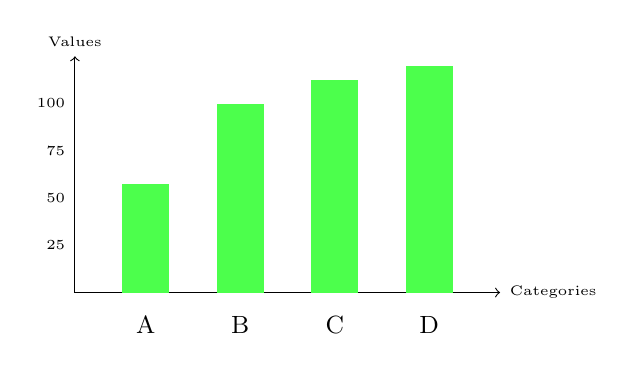
\begin{tikzpicture}[scale=0.6]
    \draw[->] (0,0) -- (9,0) node[right, font=\tiny] {Categories};
    \draw[->] (0,0) -- (0,5) node[above, font=\tiny] {Values};
    
    \fill[green!70] (1,0) rectangle (2,2.3);
    \fill[green!70] (3,0) rectangle (4,4);
    \fill[green!70] (5,0) rectangle (6,4.5);
    \fill[green!70] (7,0) rectangle (8,4.8);
    
    \node[below, font=\small] at (1.5,-0.3) {A};
    \node[below, font=\small] at (3.5,-0.3) {B};
    \node[below, font=\small] at (5.5,-0.3) {C};
    \node[below, font=\small] at (7.5,-0.3) {D};
    
    \foreach \y/\label in {1/25, 2/50, 3/75, 4/100}
        \node[left, font=\tiny] at (0,\y) {\label};
\end{tikzpicture}
\end{center}
\end{columns}
\end{frame}

\begin{frame}[fragile]{Multiple Curves - Sine/Cosine Example}
\begin{columns}[T]
\column{0.48\textwidth}
\begin{lstlisting}
import numpy as np
import matplotlib.pyplot as plt

x = np.linspace(0, 10, 100)
y1 = np.sin(x)
y2 = np.cos(x)

plt.plot(x, y1, label='Sine', 
         color='blue', linewidth=2)
plt.plot(x, y2, label='Cosine', 
         color='red', linestyle='--', 
         linewidth=2)

plt.xlabel('X')
plt.ylabel('Y')
plt.title('Trig Functions')
plt.legend()
plt.grid(True)
plt.show()
\end{lstlisting}

\column{0.48\textwidth}
\textbf{Result:}
\begin{center}
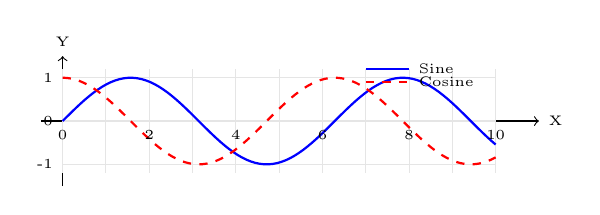
\begin{tikzpicture}[scale=0.55]
    \draw[->] (-0.5,0) -- (11,0) node[right, font=\tiny] {X};
    \draw[->] (0,-1.5) -- (0,1.5) node[above, font=\tiny] {Y};
    
    \draw[gray!20, step=1] (0,-1.2) grid (10,1.2);
    
    \draw[blue, thick, domain=0:10, samples=100] 
        plot (\x, {sin(\x r)});
    
    \draw[red, thick, dashed, domain=0:10, samples=100] 
        plot (\x, {cos(\x r)});
    
    \foreach \x in {0,2,4,6,8,10}
        \node[below, font=\tiny] at (\x,0) {\x};
    \foreach \y in {-1,0,1}
        \node[left, font=\tiny] at (0,\y) {\y};
    
    \draw[blue, thick] (7,1.2) -- (8,1.2);
    \node[right, font=\tiny] at (8,1.2) {Sine};
    \draw[red, thick, dashed] (7,0.9) -- (8,0.9);
    \node[right, font=\tiny] at (8,0.9) {Cosine};
\end{tikzpicture}
\end{center}
\end{columns}
\end{frame}

\begin{frame}[fragile]{Customization}
\begin{lstlisting}
# Colors
plt.plot(x, y, color='red')  # or 'r', '#FF0000'

# Line styles
plt.plot(x, y, linestyle='--')  # '--', '-.', ':'

# Markers
plt.scatter(x, y, marker='o')  # 'o', 's', '^', '*'

# Size
plt.plot(x, y, linewidth=3)
plt.scatter(x, y, s=100)

# Transparency
plt.scatter(x, y, alpha=0.5)  # 0 to 1
\end{lstlisting}
\end{frame}

\begin{frame}[fragile]{Chart Types - Box Plot}
\begin{columns}[T]
\column{0.48\textwidth}
\textbf{Code:}
\begin{lstlisting}
import matplotlib.pyplot as plt
import numpy as np

data = [np.random.normal(0, std, 
        100) for std in 
        range(1, 4)]

plt.boxplot(data, 
            labels=['A', 'B', 'C'])
plt.xlabel('Groups')
plt.ylabel('Values')
plt.title('Boxplot')
plt.show()
\end{lstlisting}

\column{0.48\textwidth}
\textbf{Result:}
\begin{center}
\begin{tikzpicture}[scale=0.6]
    \draw[->] (0,0) -- (8,0) node[right, font=\tiny] {Groups};
    \draw[->] (0,-4) -- (0,4) node[above, font=\tiny] {Values};
    
    \draw[thick] (1.5,-0.5) rectangle (2.5,0.5);
    \draw[thick] (2,-0.5) -- (2,0.5);
    \draw[thick] (2,-1.5) -- (2,-0.5);
    \draw[thick] (2,0.5) -- (2,1.5);
    \draw[thick] (1.8,-1.5) -- (2.2,-1.5);
    \draw[thick] (1.8,1.5) -- (2.2,1.5);
    
    \draw[thick] (3.5,-1) rectangle (4.5,1);
    \draw[thick] (4,-1) -- (4,1);
    \draw[thick] (4,-2.5) -- (4,-1);
    \draw[thick] (4,1) -- (4,2.5);
    \draw[thick] (3.8,-2.5) -- (4.2,-2.5);
    \draw[thick] (3.8,2.5) -- (4.2,2.5);
    
    \draw[thick] (5.5,-1.5) rectangle (6.5,1.5);
    \draw[thick] (6,-1.5) -- (6,1.5);
    \draw[thick] (6,-3) -- (6,-1.5);
    \draw[thick] (6,1.5) -- (6,3);
    \draw[thick] (5.8,-3) -- (6.2,-3);
    \draw[thick] (5.8,3) -- (6.2,3);
    
    \node[below, font=\small] at (2,-4.3) {A};
    \node[below, font=\small] at (4,-4.3) {B};
    \node[below, font=\small] at (6,-4.3) {C};
\end{tikzpicture}
\end{center}
\end{columns}
\end{frame}

\begin{frame}[fragile]{Subplots - Example}
\begin{columns}[T]
\column{0.5\textwidth}
\begin{lstlisting}
fig, axes = plt.subplots(2, 2, 
                    figsize=(10, 8))

# Plot 1
axes[0, 0].plot(x, y1)
axes[0, 0].set_title('Line')

# Plot 2
axes[0, 1].scatter(x, y2)
axes[0, 1].set_title('Scatter')

# Plot 3
axes[1, 0].hist(data, bins=20)
axes[1, 0].set_title('Histogram')

# Plot 4
axes[1, 1].bar(cat, val)
axes[1, 1].set_title('Bar')

plt.tight_layout()
plt.show()
\end{lstlisting}

\column{0.48\textwidth}
\textbf{Result:}
\begin{center}
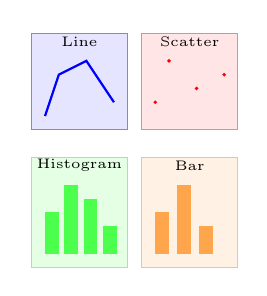
\begin{tikzpicture}[scale=0.35]
    \draw[blue!50, fill=blue!10] (0,5) rectangle (3.5,8.5);
    \draw[blue, thick] (0.5,5.5) -- (1,7) -- (2,7.5) -- (3,6);
    \node[font=\tiny] at (1.75,8.2) {Line};
    
    \draw[red!50, fill=red!10] (4,5) rectangle (7.5,8.5);
    \fill[red] (4.5,6) circle (2pt);
    \fill[red] (5,7.5) circle (2pt);
    \fill[red] (6,6.5) circle (2pt);
    \fill[red] (7,7) circle (2pt);
    \node[font=\tiny] at (5.75,8.2) {Scatter};
    
    \draw[green!50, fill=green!10] (0,0) rectangle (3.5,4);
    \fill[green!70] (0.5,0.5) rectangle (1,2);
    \fill[green!70] (1.2,0.5) rectangle (1.7,3);
    \fill[green!70] (1.9,0.5) rectangle (2.4,2.5);
    \fill[green!70] (2.6,0.5) rectangle (3.1,1.5);
    \node[font=\tiny] at (1.75,3.7) {Histogram};
    
    \draw[orange!50, fill=orange!10] (4,0) rectangle (7.5,4);
    \fill[orange!70] (4.5,0.5) rectangle (5,2);
    \fill[orange!70] (5.3,0.5) rectangle (5.8,3);
    \fill[orange!70] (6.1,0.5) rectangle (6.6,1.5);
    \node[font=\tiny] at (5.75,3.7) {Bar};
\end{tikzpicture}
\end{center}
\end{columns}
\end{frame}

\begin{frame}[fragile]{Visualizing with Pandas}
\begin{lstlisting}
import pandas as pd
import matplotlib.pyplot as plt

df = pd.read_csv('iris.csv')

# Histogram of a column
df['sepal_length'].hist(bins=20)
plt.show()

# Scatter plot
df.plot.scatter(x='sepal_length', y='sepal_width')
plt.show()

# Box plot by group
df.boxplot(column='petal_length', by='species')
plt.show()
\end{lstlisting}
\end{frame}

\begin{frame}[fragile]{Matplotlib Practice Exercise}
\begin{block}{Visualize Iris}
\begin{enumerate}
    \item Histogram for sepal\_length
    \item Scatter plot: sepal\_length vs sepal\_width
    \item Color by species
    \item 4 subplots: one histogram per feature
    \item Customize with titles, labels, colors
\end{enumerate}
\end{block}

\begin{lstlisting}
import pandas as pd
import matplotlib.pyplot as plt

df = pd.read_csv('iris.csv')
# Your code here...
\end{lstlisting}
\end{frame}

%% ========== SECTION 5 ==========
\section{Scikit-learn - First ML Model}

\begin{frame}{Scikit-learn: The ML Library}
\begin{block}{Everything for ML}
\begin{itemize}
    \item Classification algorithms
    \item Regression algorithms
    \item Clustering algorithms
    \item Data preprocessing
    \item Model evaluation
    \item Feature selection
\end{itemize}
\end{block}

\vspace{0.5cm}
\begin{center}
\textbf{A simple and consistent interface!}
\end{center}
\end{frame}

\begin{frame}{The Scikit-learn Workflow}
\begin{center}
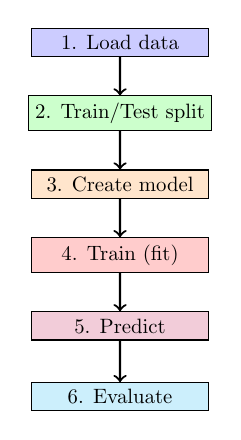
\begin{tikzpicture}[node distance=1.2cm, scale=0.75, every node/.style={scale=0.75}]
    \node[draw, rectangle, fill=blue!20, minimum width=3cm] (data) {1. Load data};
    \node[draw, rectangle, fill=green!20, minimum width=3cm, below of=data] (split) {2. Train/Test split};
    \node[draw, rectangle, fill=orange!20, minimum width=3cm, below of=split] (model) {3. Create model};
    \node[draw, rectangle, fill=red!20, minimum width=3cm, below of=model] (train) {4. Train (fit)};
    \node[draw, rectangle, fill=purple!20, minimum width=3cm, below of=train] (predict) {5. Predict};
    \node[draw, rectangle, fill=cyan!20, minimum width=3cm, below of=predict] (eval) {6. Evaluate};
    
    \draw[->, thick] (data) -- (split);
    \draw[->, thick] (split) -- (model);
    \draw[->, thick] (model) -- (train);
    \draw[->, thick] (train) -- (predict);
    \draw[->, thick] (predict) -- (eval);
\end{tikzpicture}
\end{center}
\end{frame}

\begin{frame}[fragile]{Iris Classification (1/3)}
\begin{lstlisting}
# 1. Imports
from sklearn.datasets import load_iris
from sklearn.model_selection import train_test_split
from sklearn.neighbors import KNeighborsClassifier
from sklearn.metrics import accuracy_score

# 2. Load the data
iris = load_iris()
X = iris.data   # Features (4 columns)
y = iris.target # Labels (species: 0, 1, 2)

print("X shape:", X.shape)  # (150, 4)
print("y shape:", y.shape)  # (150,)
\end{lstlisting}
\end{frame}

\begin{frame}[fragile]{Iris Classification (2/3)}
\begin{lstlisting}
# 3. Split into train/test (80/20)
X_train, X_test, y_train, y_test = train_test_split(
    X, y, test_size=0.2, random_state=42
)

print("Train:", X_train.shape)  # (120, 4)
print("Test:", X_test.shape)    # (30, 4)

# 4. Create the model
model = KNeighborsClassifier(n_neighbors=3)

# 5. Train
model.fit(X_train, y_train)
print("Model trained!")
\end{lstlisting}
\end{frame}

\begin{frame}[fragile]{Iris Classification (3/3)}
\begin{lstlisting}
# 6. Predictions
y_pred = model.predict(X_test)

# 7. Evaluate
accuracy = accuracy_score(y_test, y_pred)
print(f"Accuracy: {accuracy * 100:.2f}%")

# Look at a few predictions
print("\nExamples:")
for i in range(5):
    print(f"Actual: {y_test[i]}, Predicted: {y_pred[i]}")
\end{lstlisting}

\vspace{0.3cm}
\begin{block}{Result}
Accuracy: 96-100\% on Iris!
\end{block}
\end{frame}

\begin{frame}[fragile]{Standard Sklearn Structure}
\begin{lstlisting}
from sklearn.whatever import MyModel

# 1. Create the model
model = MyModel(parameters)

# 2. Train
model.fit(X_train, y_train)

# 3. Predict
predictions = model.predict(X_test)

# 4. Evaluate
from sklearn.metrics import accuracy_score
score = accuracy_score(y_test, predictions)
\end{lstlisting}

\begin{alertblock}{Important}
The same structure applies to ALL sklearn algorithms!
\end{alertblock}
\end{frame}

\begin{frame}[fragile]{Preprocessing}
\begin{lstlisting}
from sklearn.preprocessing import StandardScaler

# Normalize (mean=0, std=1)
scaler = StandardScaler()

# Fit on train, transform train and test
X_train_scaled = scaler.fit_transform(X_train)
X_test_scaled = scaler.transform(X_test)

# Use the normalized data
model.fit(X_train_scaled, y_train)
predictions = model.predict(X_test_scaled)
\end{lstlisting}

\vspace{0.3cm}
\begin{block}{Why?}
Some algorithms are sensitive to scale!
\end{block}
\end{frame}

\begin{frame}[fragile]{Application Exercise}
\begin{block}{Your First Model}
\begin{enumerate}
    \item Load the Iris dataset
    \item Split into train (70\%) and test (30\%)
    \item Train a KNN with k=5
    \item Make predictions
    \item Compute and display accuracy
    \item Show a few predictions vs actual values
\end{enumerate}
\end{block}

\begin{lstlisting}
from sklearn.datasets import load_iris
from sklearn.model_selection import train_test_split
from sklearn.neighbors import KNeighborsClassifier
from sklearn.metrics import accuracy_score


\end{lstlisting}
\end{frame}

%% ========== SECTION 6 ==========
\section{Workflow and Best Practices}

\begin{frame}{Complete ML Workflow}
\begin{enumerate}
    \item \textbf{Understand the problem}
    \begin{itemize}
        \item Classification? Regression? Clustering?
    \end{itemize}
    
    \item \textbf{Explore the data}
    \begin{itemize}
        \item df.info(), df.describe(), visualizations
    \end{itemize}
    
    \item \textbf{Prepare the data}
    \begin{itemize}
        \item Missing values, normalization
    \end{itemize}
    
    \item \textbf{Train a model}
    \begin{itemize}
        \item Start simple (KNN, trees...)
    \end{itemize}
    
    \item \textbf{Evaluate and improve}
    \begin{itemize}
        \item Metrics, cross-validation
    \end{itemize}
\end{enumerate}
\end{frame}

\begin{frame}[fragile]{Complete Template (1/2)}
\begin{lstlisting}
import pandas as pd
import numpy as np
import matplotlib.pyplot as plt
from sklearn.model_selection import train_test_split
from sklearn.preprocessing import StandardScaler
from sklearn.neighbors import KNeighborsClassifier
from sklearn.metrics import accuracy_score

# 1. Load
df = pd.read_csv('data.csv')

# 2. Explore
print(df.head())
print(df.info())
df.hist()
plt.show()
\end{lstlisting}
\end{frame}

\begin{frame}[fragile]{Complete Template (2/2)}
\begin{lstlisting}
# 3. Prepare
X = df.drop('target', axis=1).values
y = df['target'].values

# 4. Split
X_train, X_test, y_train, y_test = train_test_split(
    X, y, test_size=0.2, random_state=42)

# 5. Normalize
scaler = StandardScaler()
X_train = scaler.fit_transform(X_train)
X_test = scaler.transform(X_test)

# 6. Train
model = KNeighborsClassifier(n_neighbors=5)
model.fit(X_train, y_train)

# 7. Evaluate
y_pred = model.predict(X_test)
print(f"Accuracy: {accuracy_score(y_test, y_pred):.2f}")
\end{lstlisting}
\end{frame}


\begin{frame}{Resources}
\begin{block}{Documentation}
\begin{itemize}
    \item NumPy: numpy.org/doc
    \item Pandas: pandas.pydata.org/docs
    \item Matplotlib: matplotlib.org
    \item Scikit-learn: scikit-learn.org
\end{itemize}
\end{block}

\begin{block}{Practice}
\begin{itemize}
    \item Kaggle: datasets and tutorials
    \item Google Colab: free notebooks
    \item UCI ML Repository: datasets
\end{itemize}
\end{block}
\end{frame}

\begin{frame}{Recap}
\begin{block}{You now know}
\begin{itemize}
    \item \textbf{NumPy}: fast numerical computation
    \item \textbf{Pandas}: data manipulation
    \item \textbf{Correlation}: interpreting relationships
    \item \textbf{Matplotlib}: visualization
    \item \textbf{Scikit-learn}: ML models
\end{itemize}
\end{block}

\vspace{0.5cm}
\begin{alertblock}{Next Step}
Classification algorithms!
\end{alertblock}
\end{frame}



\end{document}
